\documentclass[11pt, oneside]{article}   	% use "amsart" instead of "article" for AMSLaTeX format
\usepackage{geometry}                		% See geometry.pdf to learn the layout options. There are lots.
\geometry{letterpaper}                   		% ... or a4paper or a5paper or ... 
%\geometry{landscape}                		% Activate for for rotated page geometry
%\usepackage[parfill]{parskip}    		% Activate to begin paragraphs with an empty line rather than an indent
\usepackage{graphicx}				% Use pdf, png, jpg, or eps� with pdflatex; use eps in DVI mode
								% TeX will automatically convert eps --> pdf in pdflatex		
\usepackage{amssymb}
\usepackage{amsmath}
\usepackage{parskip}
\usepackage{color}

\title{Shankar Problem Set 1-1}
%\author{The Author}
%\section{}
% \subsection*{R code}
\date{}							% Activate to display a given date or no date

\graphicspath{{/Users/telliott_admin/Dropbox/Tex/png/}}

% \begin{center} 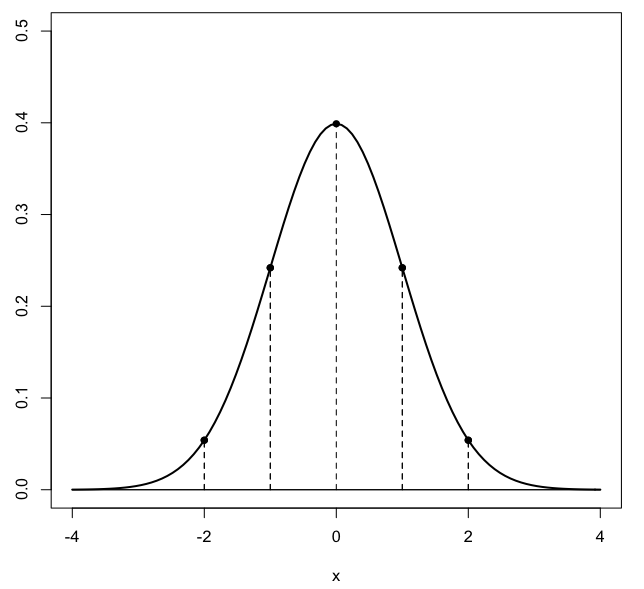
\includegraphics [scale=0.4] {gauss3.png} \end{center}

\begin{document}
\maketitle
\Large
\noindent


A ball $A$ falls from a height $H$, starting at the same time as ball $B$ is thrown upward from the ground with velocity $v^*$.  At impact, $v_A = 2 v_B$.  Find the height at impact $h$ as ratio to $H$.  Assume $a = -g = -10$ m/s${^2}$.
\[ y = y_0 + v^* t + \frac{1}{2}at^2 \]
\[ y_A = H + 0 -5 t^2 \]
\[ y_B = 0 + v^* t -5 t^2 \]
At impact
\[ y_A = y_B \]
\[ H = v^*t \]
We also have that
\[ v = v_0 + at \]
\[ v_A = at = -10t \]
\[ v_B = v^* + at = v^* - 10t \]
At impact
\[ v_A = 2 v_B \]
\[ -10t = 2v^* - 20 t \]
\[ 5t = v^* \]
\[ t = \frac{v^*}{5} \]
Substitute for $t$ above
\[ H = v^*t = 5t^2 \]
\[ t = \sqrt{\frac{H}{v^*}} \]
Check that $y_A = y_B$
\[ y_A = H - 5 t^2 = H - H = 0 \]
\[ y_B = v^* t - 5 t^2 = H - H = 0 \]
And the velocities are
\[ v_A = -10t = -10 \frac{v^*}{5} = -2 v^* \]
\[ v_B =  v^* - 10t = v^* + v_A = - v^* = \frac{1}{2} v_A \]




\end{document}  